\chapter{Auswertung}

\section{Dopplerverbreitertes Spektrum}

\begin{figure}[ht]
  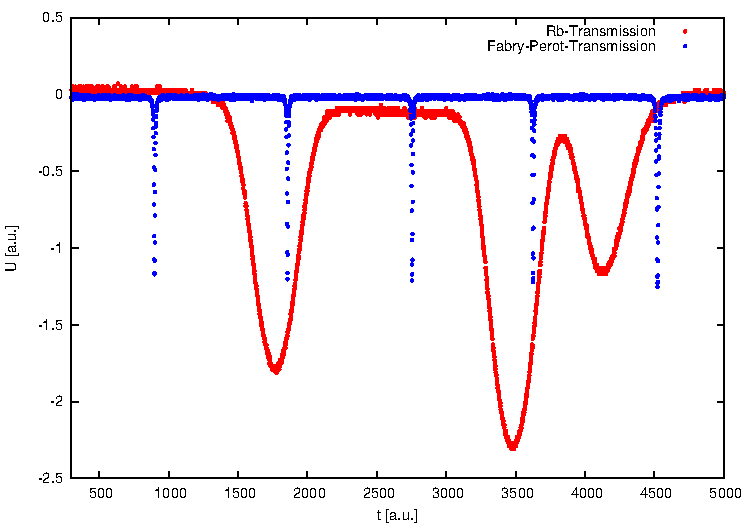
\includegraphics[width=0.9\textwidth]{./dopplerspektrum-messung.pdf}
  \caption{Die Spannung der differentiellen Photodiode (proportional zur Intensit�t
  		    des durch die Rb-Zelle transmittierten Lichts in willk�rlichen Einheiten)
			und entsprechend die Spannung hinter dem Fabry-P�rot-Resonator
		    aufgetragen gegen die Zeit $t$, w�hrend der der Frequenzbereich des Lasers 
			durchgefahren wird, ebenfalls in willk�rlichen Einheiten.}
\label{fig:dopplerroh}
\end{figure}

In Abbildung \ref{fig:dopplerroh} sind die vom Oszilloskop aufgenommenen Messdaten
dargestellt. Zu sehen sind von links nach rechts die 85F2-, 85F3- und 87F2-Resonanzen
(85F2 heisst hier z.B. die �berlagerung der drei �berg�nge vom $F=2$--Grundniveau des
$^{85}\text{Rb}$--Isotops)

Die Resonanzen des Fabry-P�rot-Signals entsprechen konstanten Frequenzabst�nden und dies
wird als Grundlage f�r einen Fit durch ein Polynom dritten Grades $f$ genutzt
(f�nf Messpunkte $(t_i,f(t_i))$ bei den Zeitpunkten $t_i$ der Resonanzen mit
gleichem $f(t)$-Abstand), siehe Abbildung \ref{fig:xumskalierung}.
\begin{figure}[!ht]
  \includegraphics[width=1\textwidth]{./xumskalierung.pdf}
  \caption{Umskalierung der Messzeitachse zur Frequenzachse}
\label{fig:xumskalierung}
\end{figure}
Wenn dann das Dopplerspektrum $I$ gegen $f(t)$ aufgetragen wird, stimmt die Skalierung
bis auf eine lineare Umskalierung, die abschliessend durch Kenntnis der Position und
Abst�nde der Spektrallinien erfolgt. Vor dieser linearen Umskalierung werden die
$(I,f(t))$--Daten durch eine Summe von zwei �berlagerungen f�r die 85F2- und
85F3-Resonanzen
aus jeweils drei Gau�profilen
mit gleicher Breite (die nach \eqref{eq:gausstemp} der Temperatur des Rb-Gases entspricht)
und durch Literaturwerte [2] vorgegebene Amplitudenverh�ltnisse und einer beliebigen
Gau�funktion f�r die rechte 87F2-Resonanz gefittet.

\begin{figure}[ht]
  \includegraphics[width=1\textwidth]{./dopplerfit-plot.pdf}
  \caption{Gemessenes Dopplerspektrum in willk�rlichen Einheiten gegen die
  		umskalierte $f(t)$--Achse in Schwarz; Fit in Rot}
\label{fig:dopplerfit}
\end{figure}

Aus dem Fit ergibt sich eine gemeinsame halbe $\frac{1}{e}$--Breite $w$ der �berlagerten
Gau�profile f�r die 85F2- und 85F3-Resonanzen in Einheiten der $f(t)$--Achse als Parameter
des Fits, aus der
wir die volle Halbwertsbreite in MHz durch Umrechnung der Breitenarten
(halbe $\frac{1}{e}$--Breite in volle Halbwertsbreite) und
Skalierung erhalten, da die wahren relativen
Abst�nde der Resonanzen aus der Literatur [2] bekannt sind.

Wir erhalten somit:
\begin{equation}
	w = (406,5 \pm 0,8) \text{ MHz}
\end{equation}

Mit Gleichung \eqref{eq:gausstemp} ergibt sich daraus f�r die Temperatur des Rb-Gases
\begin{equation}
	T = (434,46 \pm 1,7) \text{ K}
\end{equation}



\section{Dopplerfreie S�ttigungsspektroskopie}

\subsection{Messung der Strahlgr��e}

